\chapter{PHOEBE Gráficas Adicionales} \label{apendice:modelo_computacional_graficas}

\section{Distribuciones Priores Completas} \label{apendice:modelo_computacional_graficas:dist_priores_completas}

\begin{figure}[!ht]
    \centering
    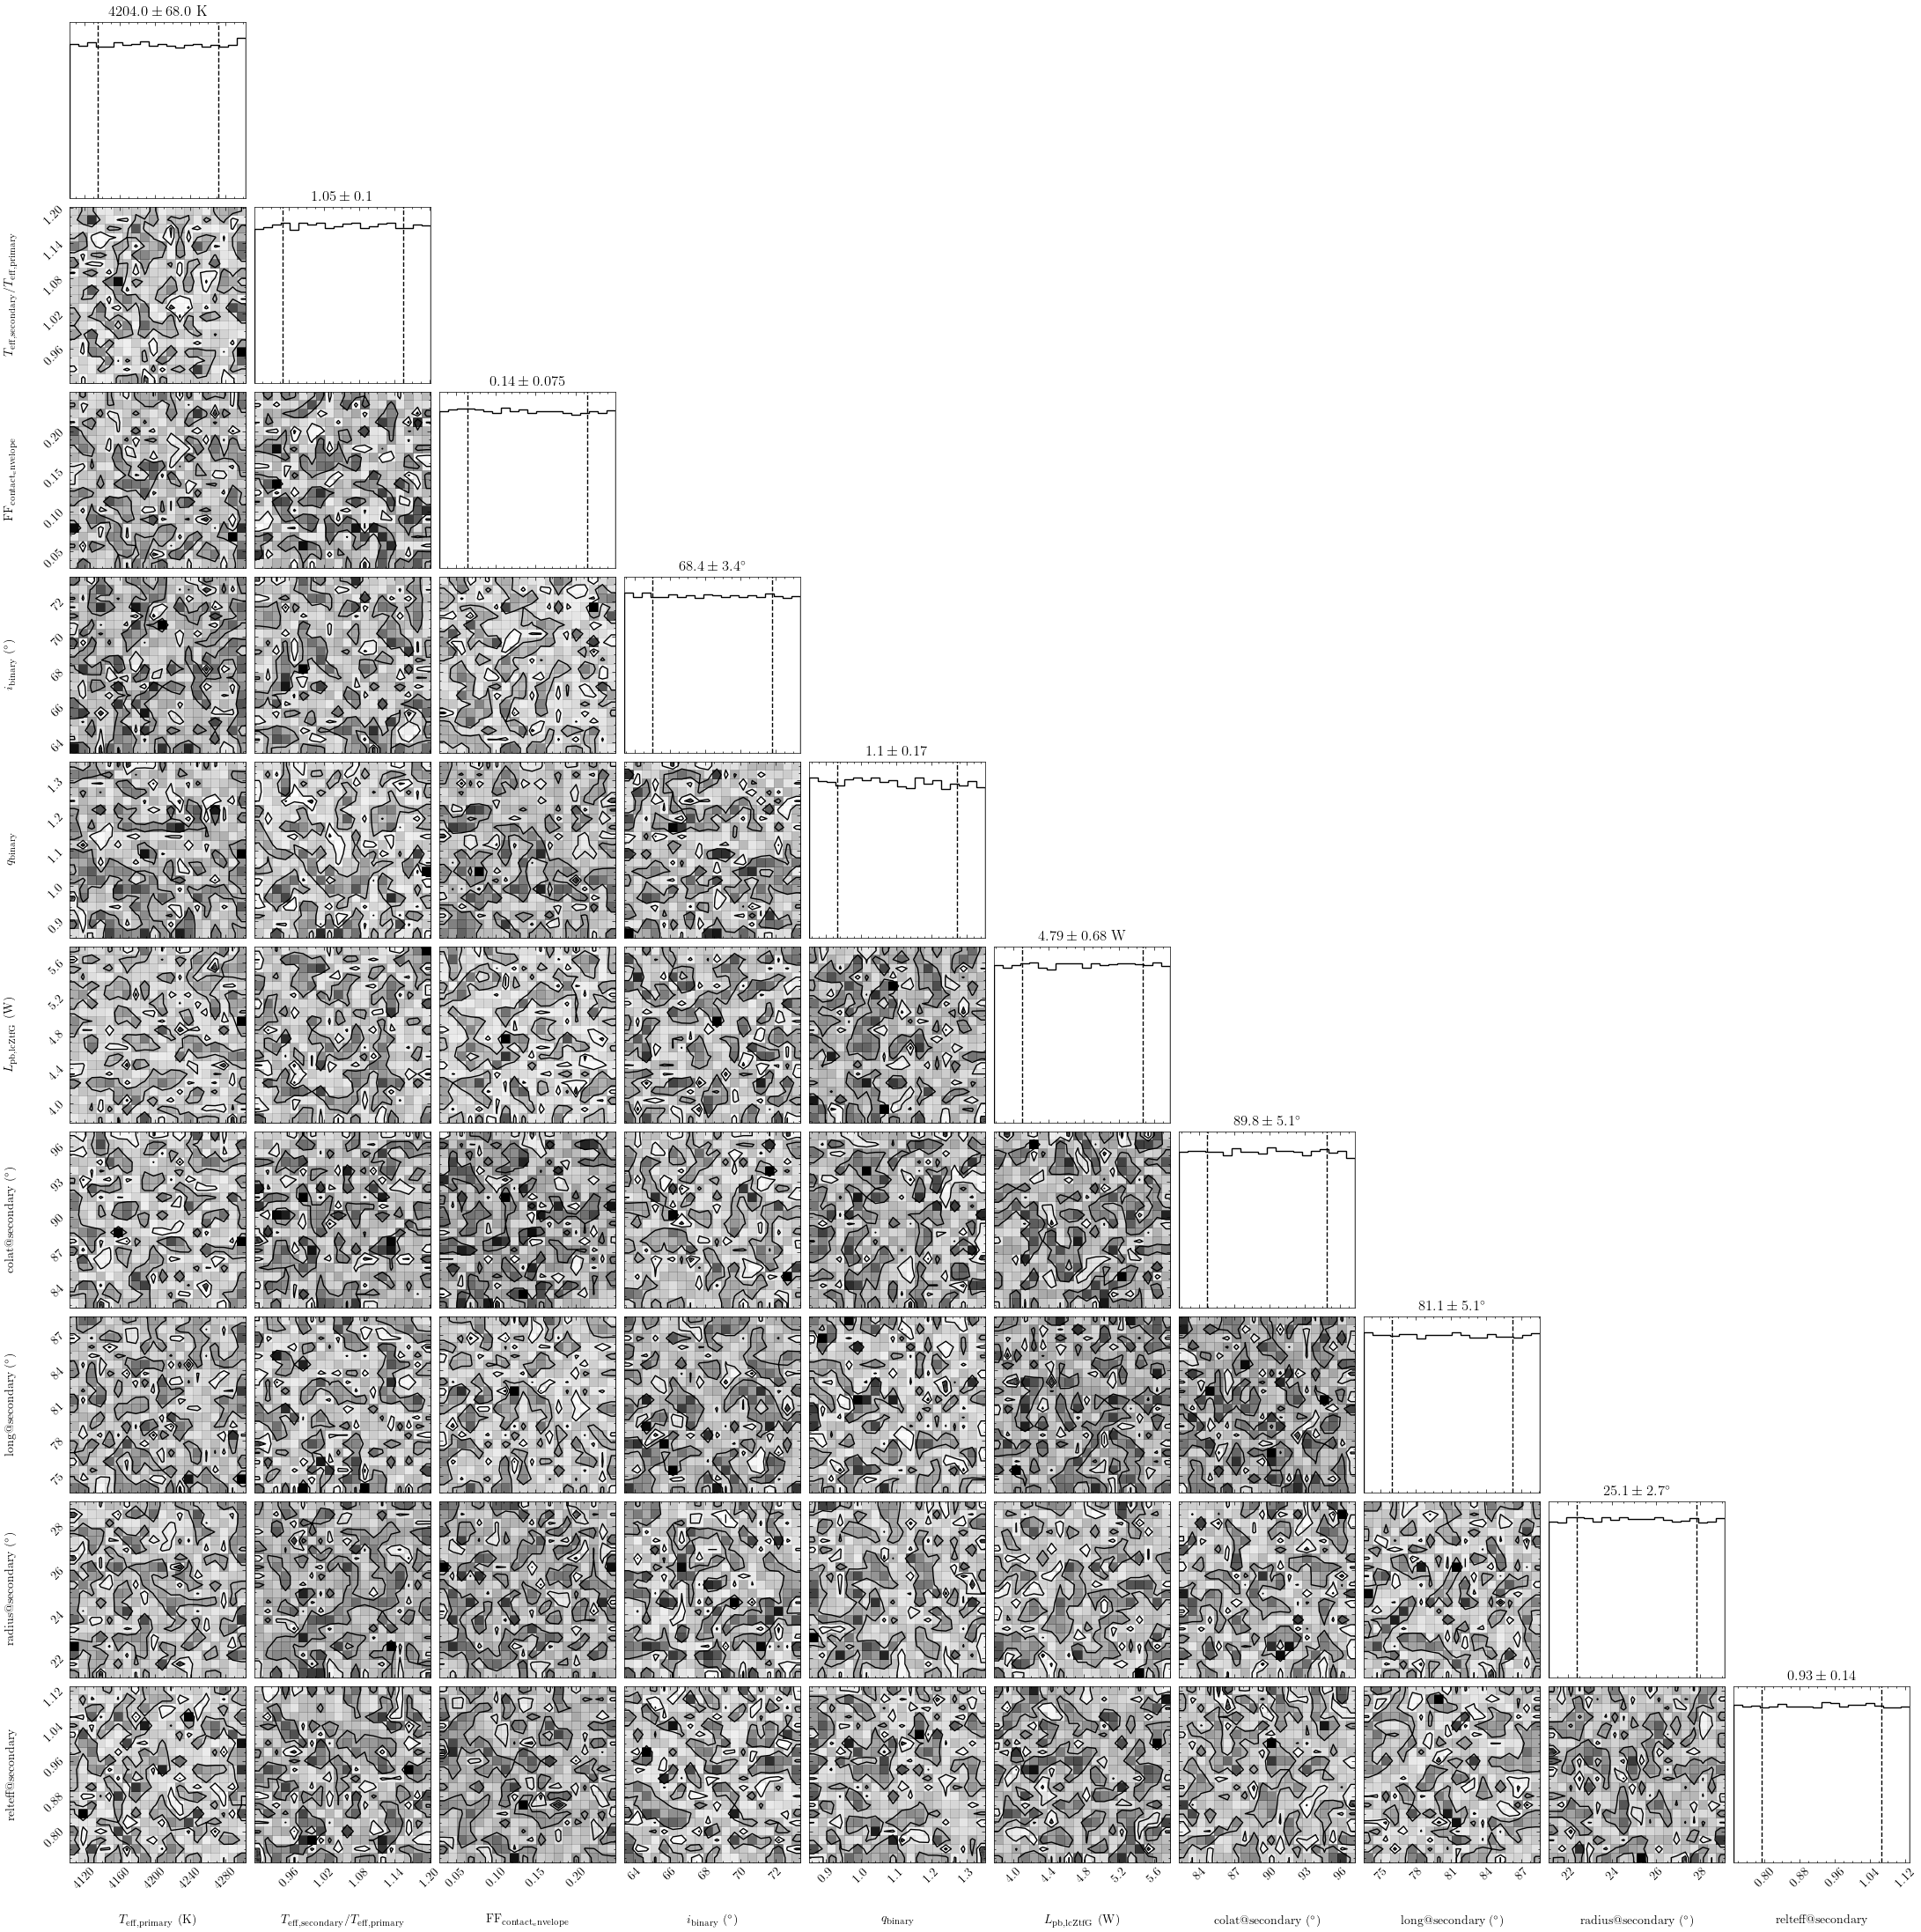
\includegraphics[scale=0.255]{Metodologia/Secciones/ModeloComputacional/Figures/Figura Prior Params Combinadas.png}
    \caption{Distribuciones uniformes de todos los parámetros muestreados
    utilizando cadenas de Monte Carlo (MCMC). La topología compleja que se ve en
    cada cuadrante se debe a las muestras que PHOEBE toma para cada parámetro en
    el proceso de generar la gráfica, no debido a la distribución almacenada por
    PHOEBE. Los priores, junto a esta gráfica, fueron generados en el Notebook
    \href{https://github.com/KnightIV/UANL_MAPTA_Observaciones/blob/main/analisis/phoebe_model/sampling/updated-data-mcmc-sampling.ipynb}{\code{updated-data-mcmc-sampling.ipynb}}.}
    \label{figuraPhoebePrioresCombinadasZtf}
\end{figure}